
\documentclass[12pt]{article}
\usepackage[a4paper, margin=.30in]{geometry}
\usepackage{graphicx ,
            wrapfig,
            xcolor, 
            enumerate,
            amsmath,
			fontenc,
			tcolorbox
            }

\newcommand\headerMe[2]{\noindent{}#1\hfill#2}
\renewcommand{\thesection}{\Roman{section}}

\author{Zakaria HAOUZAN}
\date{\today}

\begin{document}
% headers --------------
\headerMe{Matière : Physique-Chimie}{Professeur : Zakaria HAOUZAN}\\
\headerMe{Unité : Travail Mécanique et Energie }{Établissement : Lycée SKHOR qualifiant}\\
\headerMe{Niveau : 2BAC-SM-X}{Heure : 5H}\\

% ------Content ________
\begin{center}

    \Large{Leçon $N^{\circ} 2 $: \color{red}Ondes mécaniques progressives périodiques. }
\end{center}


\section{Notion d’onde mécanique progressive périodique}
\subsection{Définition : }

\begin{wrapfigure}[5]{r}{0.15\textwidth}
	\vspace{-2cm}
	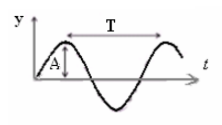
\includegraphics[width=0.15\textwidth]{./img/OMPsins.png}
	\caption{ onde mécanique périodique sinusoïdale}
\end{wrapfigure}

Une onde est périodique si elle se répète indentiquement à elle-même pendant des mêmes intervalles de temps appellés période T .  

Elle est dite sinusoïdale si sa variation est une sinusoïde en fonction du temps et l'élongation d'un point du milieu de propagation
s'écrit de la manière suivante: \\$y(t) = Asin(\frac{2.\pi}{T}.t + \phi)$

\vspace{-0.4cm}
\begin{itemize}
\item y(t): l’élongation à un instant t en (m).
\item A : l'amplitude (élongation maximale ) en (m).
\item T : la période (périodicité temporaire) et la frequence  $\nu = \frac{1}{T}$ (Hz).
\item la phase à l'origine, elle se détermine à partir des conditions initiales (en rad).
\end{itemize}

\subsection{Exemple 1:Périodicité temporelle }
En produisant un son à l'aide d'un haut parleur lié à un générateur (GBF) devant un microphone lié à un oscilloscope on obtient
l'enregistrement suivant:
\begin{figure}[h]
	\begin{center}
		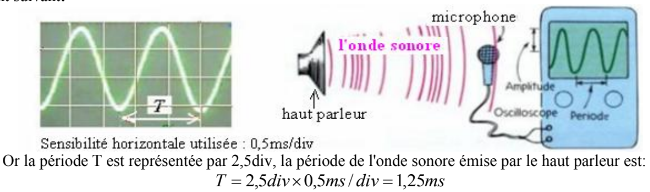
\includegraphics[width=0.6\textwidth]{./img/OMPPExemple1.png}
	\end{center}
\end{figure}
\begin{center}
	\vspace{-2.5cm}
\end{center}

\subsection{Exemple 2:Périodicité spatiale.}

La stroboscopie est une méthode d'observation d'un mouvement en utilisant le stroboscope qui est un appareil qui émet des éclairs
périodiques selon des fréquences réglables.
\begin{figure}[h]
	\begin{center}
	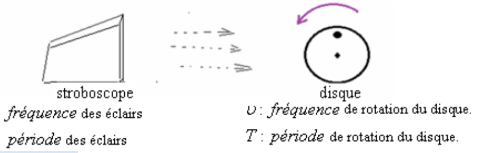
\includegraphics[width=0.5\textwidth]{./img/OMPPstroposcope.png}
\end{center}
\end{figure}

Durant la rotation le disque apparaît blanc, l'œil ne peut pas suivre le mouvement de la tâche et lorsqu'on l'éclaire avec le
stroboscope on s'intéresse aux trois cas suivants : \underline{l'immobilité apparente} et le mouvement apparent ralenti dans le même sens puis
celui dans le sens contraire du mouvement de rotation du disque et cela suivant les fréquences du stroboscope.

\textbf{\underline{Dans le cas de l'immobilité apparente :}}on observe que la tâche est immobile car elle est éclairée au même endroit.

\begin{figure}[h]
	\begin{center}
	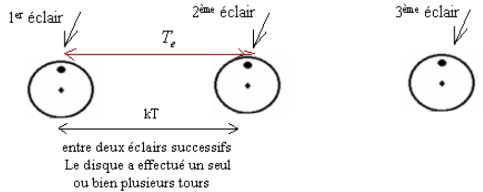
\includegraphics[width=0.5\textwidth]{./img/OMPPimmobilité apparente.png}
\end{center}
\vspace{-1.2cm}
\end{figure}

La relation entre la période des éclairs et celle de rotation du disque.$Te=kT$ avec $k\in N*$  donc $\nu = k\nu_e$

La plus grande fréquence des éclaires qui permet d'avoir l'immobilité apparente correspond à $k=1$ donc: $\nu=\nu_e$.

\textbf{\underline{Cas du mouvement ralenti apparent :}} -On obtient un mouvement ralenti apparent dans le même sens de rotation du disque si $\nu_e$ est est légèrement inférieure à $\nu$.

-On obtient un mouvement ralenti apparent dans le sens contraire de rotation du disque si $\nu_e$ est légèrement supérieure à $\nu$.

\section{Exemples d'ondes mécaniques progressives périodiques : }
\subsection{Onde progressive le long d'une corde : }
On utilise une corde élastique tendue horizontalement par un corps suspendu comme l'indique la figure suivante .La corde est attachée en S au bout d'une lame vibrante dont le mouvement est entretenu par un électro-aimant alimenté par un courant alternatif.

\begin{figure}[h]
	\begin{center}
\vspace{-0.5cm}
	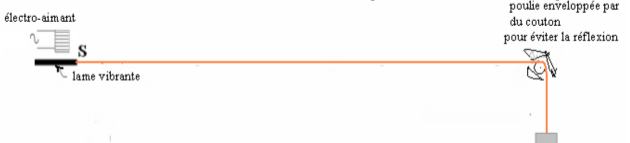
\includegraphics[width=0.66\textwidth]{./img/OMPPExperience.png}
\end{center}
\vspace{-2cm}
\end{figure}

Lorsque la lame vibre avec une fréquence $\nu = 100Hz$, la corde parait floue,ce qui prouve que tous ses points sont en mouvement.

En utilisant le stroboscope et en le réglant sur la fréquence $\nu_e = \nu =100Hz$, on obtient le mouvement apparent ralenti dans le sens contraire de celui de propagation de l'onde.
\begin{figure}[h]
	\begin{center}
\vspace{-0.5cm}
	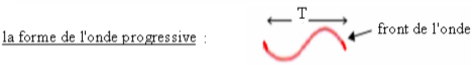
\includegraphics[width=0.46\textwidth]{./img/OMPPexProg.png}
\end{center}
\vspace{-1cm}
\end{figure}

\begin{wrapfigure}[10]{r}{0.27\textwidth}
	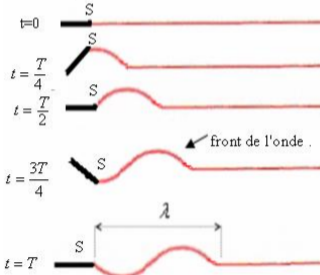
\includegraphics[width=0.29\textwidth]{./img/OMPPtimes.png}
\end{wrapfigure}


T: périodicité temporaire (période de l'onde progressive)

Faisons des représentations successives de l'aspect de la corde pendant des intervalles de temps successifs et égaux à T/4 (T étant la période de vibration de la source) :
$\lambda $: Longueur d'onde (périodicité spatiale).

\subsubsection{Définition de la Longueur d'onde : }
La longueur d'onde est la distance parcourue par l'onde pendant une période T. $$\lambda = v.T = \frac{v}{\nu}$$
$\lambda:$ Longueur d'onde (m)  $v$: célérité de propagation de l'onde (m/s)  $\nu$: fréquence de l'onde progressive (Hz)
\begin{figure}[!h]
	\begin{center}
    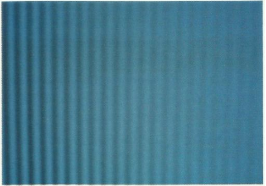
\includegraphics[width=0.3\textwidth]{./img/OMPPrectilgne.png}
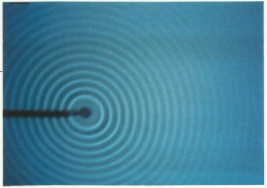
\includegraphics[width=0.3\textwidth]{./img/OMPPcirculaire.png}
    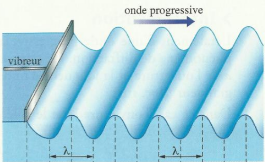
\includegraphics[width=0.3\textwidth]{./img/OMPPdemo.png}
\end{center}
\end{figure}


\subsection{Onde progressive à la surface de l'eau : }

On provoque une onde dans une cuve à onde par une source vibrante .Pour obtenir l'immobilité apparente on éclair la surface de l'eau par un stroboscope dont la fréquence est réglée sur une valeur égale à la fréquence de vibration de l'onde progressive c'est-à-dire celle de la source vibrante .On obtient par stroboscopie la figure suivante.


\begin{tcolorbox}

Toute onde périodique progressive présente une double périodicité:
  
une périodicité temporelle de période T;
  
une périodicité spatiale de période,appelée longueur d'onde.
\end{tcolorbox}

\subsubsection{Application 1:}
Sachant que la célérité de propagation de l’onde est $v=2,5m/s$ et la longueur de l’onde progressive est
$\lambda = 1cm$. Quelle est la fréquence de vibration de la source?


\subsubsection{Application 2:}
Dans l’expérience précédente, sachant que la plus grande fréquence du stroboscope qui permet d’obtenir l’immobilité apparente
est 250Hz.

En mesurant la longueur de l'onde progressive on obtient $\lambda=0.8cm$.

a) Quelle est la fréquence de l’onde progressive ? Justifier votre réponse.

b) Déterminer la célérité de propagation de l’onde progressive.

\subsection{Ondes sonores et ultrasonores : }
\begin{tcolorbox}
a - Les ondes sonores:
Les ondes sonores sont des ondes mécaniques périodiques longitudinales résultant de la compression et la dilatation des
constituants du milieu de propagation.
\end{tcolorbox}

\begin{tcolorbox}
b -Les ondes ultrasonores sont des ondes sonores dont la fréquence est supérieure à 20kHz, ils sont inaudibles et ils se réfléchissent
partiellement sur un obstacle.

(les ultrasons ne sont pas entendus par l’homme mais certains animaux comme les chauves souris, les dauphins ou les baleines
sont capable de les percevoir.)

\end{tcolorbox}

\section{Détermination expérimentale de la célérité de propagation d'une onde sonore : }

\subsection{Comparaison du mouvement de deux points du milieu de propagation: }
\begin{figure}[h]
	\begin{center}
\vspace{-0.5cm}
	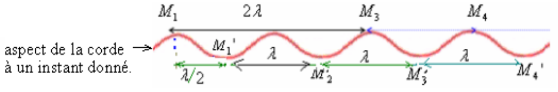
\includegraphics[width=0.56\textwidth]{./img/OMPPcelerite.png}
\end{center}
\vspace{-1cm}
\end{figure}

$M_1M_3 = 2\lambda$ , $M_1$ et $M_3$ vibrent en phase.

$M_3M_4 = \lambda$ , $M_3$ et $M_4$ vibrent en phase.

$M_1M_4 = 3\lambda$ , $M_1$ et $M_4$ vibrent en phase.

\begin{tcolorbox}
	En général,deux pointsMetM'du milieu de propagation vibrent en phase si la distance qui les sépare est un multiple de la longueur d'onde $\lambda$ : $MM' = k.\lambda$, $k\in N^*$
\end{tcolorbox}

$M_1M_1' = \frac{\lambda}{2}$ , $M_1$ et $M_1'$ vibrent en opposition de phase.

$M_1M_2' = 3\frac{\lambda}{2}$ , $M_3$ et $M_2'$ vibrent en opposition de phase.

$M_1M_3' = 5.\frac{\lambda}{2}$ , $M_1$ et $M_3'$ vibrent en opposition de phase.

\begin{tcolorbox}
	En général,deux pointsMetMdu milieu de propagation vibrent en opposition si la distance qui les sépare est un nombre impaire de la demi-longeur d'onde : $MM' = (2K' + 1 ).\frac{\lambda}{2}$ , $K' \in N$
\end{tcolorbox}

\section*{Remarque :}
\begin{tcolorbox}
	On dit que deux fonctions sinusoïdales sont en phase si elles s'annulent en même temps et elles atteignent leur
maximum et leur minimum en même temps.
\tcblower
On dit que deux fonctions sinusoïdales sont en opposition de phase si elles s'annulent en même temps mais l'une est maximale
quand l'autre est minimale.
\end{tcolorbox}

\section*{Application 3 : }


En mesurant dans une cuveàonde la longueur de l'on de progressive on trouve : $\lambda = 2cm$ Comparer le mouvement de deux points M e N du milieu de propagation dans chacun des cas suivants :

a) MN=6cm.

b) MN=7cm

\begin{wrapfigure}[4]{r}{0.3\textwidth}
	\vspace{-1cm}
	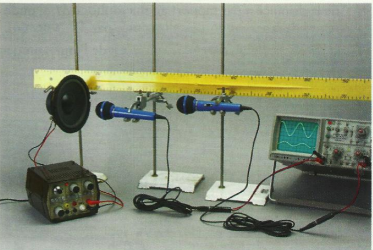
\includegraphics[width=0.3\textwidth]{./img/OMPPexprience2.png}
	\caption{Dispositif expérimental}
\end{wrapfigure}


\subsection{Expérience des deux microphones: }

Pour déterminer la vitesse de propagation du son émis par un haut-parleur dans l'air on utilise le montage suivant: Après avoir activé le haut parleur on visualise sur l'écran de l'oscilloscope le signal correspondant à chacun des microphones M1 et M2..

\begin{figure}[h]
	%\begin{center}
\vspace{-0.5cm}
	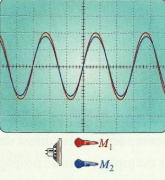
\includegraphics[width=0.2\textwidth]{./img/OMPPcas1.png}
	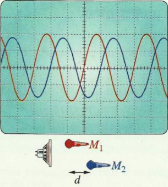
\includegraphics[width=0.2\textwidth]{./img/OMPPcas2.png}
	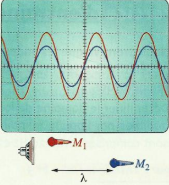
\includegraphics[width=0.2\textwidth]{./img/OMPPcas3.png}
%\end{center}
\vspace{-0.9cm}
\end{figure}

\begin{itemize}
	\item Lorsque les deux microphones sont placés côte à côte face au haut parleur et à la même distance de lui, les deux signaux correspondant à M1 et à M2 sont en phase.
	\item Pour un son de fréquence de $10^3Hz$ émis, on laisse le microphone M1 à sa place et on déplace le microphone M2 lentement et parallèlement à l'axe du haut-parleur.
	\item On indique la distance d chaque fois que les deux signaux sont en phase et on obtient les résultats suivants: d(cm) [34, 68, 102, 136].
	\item Or deux points du milieu de propagation vibrent en phase si la distance qui les sépare est un multiple de la longueur d'onde $d =k\lambda$ 
		\begin{itemize}
			\item Pour k =1, $d = \lambda = 34cm$
			\item Pour k =2,$d = 2\lambda = 68cm$
			\item Pour k =3,$d = 3\lambda = 102cm$
			\item Pour k =4,$d = 4\lambda = 136cm$
		\end{itemize}
\end{itemize}

Donc la longueur de l'onde sonore émise par le haut parleur est $\lambda=34cm$.

Elle correspondàla plus petite distancedpour laquelle les signaux sont pour la première fois en phase.

On a T=0.2ms/div x 5div = $10^{-3}$s

Elle correspondàla plus petite distancedpour laquelle les signaux sont pour la première fois en phase.

$$v = \frac{\lambda}{T} = 340m/s$$

\begin{wrapfigure}[7]{r}{0.6\textwidth}
	\vspace{-2cm}
	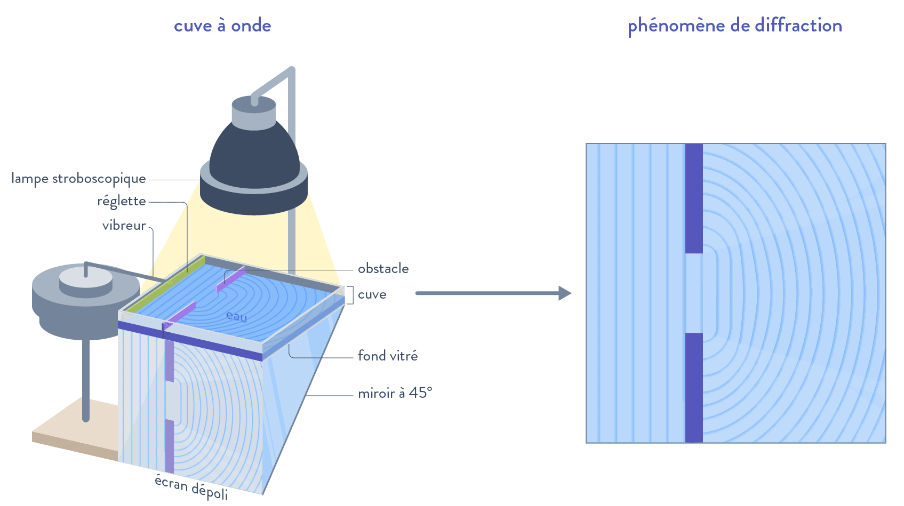
\includegraphics[width=0.6\textwidth]{./img/OMPPcuveExp.png}
	%\caption{Dispositif expérimental}
\end{wrapfigure}


\section{Phénomène de diffraction: }
\subsection{Définition}
La diffraction est un phénomène qui caractéristique des ondes, il se produit lorsque l'onde passe à travers une ouverture de taille comparable à la longueur d'onde ($a \approx \lambda$).

C'est la modification de la forme d'une onde passant par une ouverture de largeur $a \leq \lambda$.

\subsection{Onde diffractée àla surface de l'eau :}
On utilise une cuve à onde muni d'une plaque vibrante devant laquelle on place un diaphragme comportant une ouverture de largeur a. (dans la figure Onde incidente et Onde diffractée)
\begin{figure}[h]
	\begin{center}
\vspace{-0.5cm}
	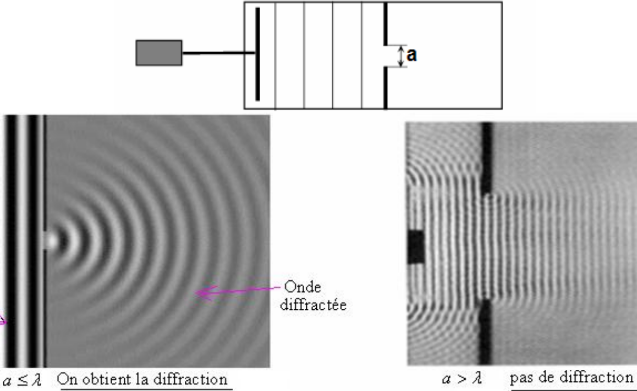
\includegraphics[width=0.5\textwidth]{./img/OMPPleaudiff.png}
\end{center}
\vspace{-0.9cm}
\end{figure}

L'ouverture se comporte comme une source ponctuelle donnant naissance à des ondes circulaires.
L'onde incidente et l'onde diffractée ont la même longueur d'onde et même célérité de propagation mais des directions de
propagation différentes.

\section{Phénomène de dispersion ++ bonus ++ } 

\begin{tcolorbox}
	\begin{itemize}
		\item Un milieu dispersif est un milieu dans lequel la vitesse de propagation d'une onde dépend de sa fréquence.

		\item  La célérité de propagation de l'onde change de valeur lorsqu'on fait varier la fréquence de vibration de la source.
La célérité de propagation de l'onde dépend de sa fréquence.
Par conséquence : l'eau est un milieu dispersif.
\item Les sons et les ultrasons ont des fréquences différentes, mais la célérité dans l'air est la même. L'air
n'est donc pas un milieu dispersif pour ces ondes.
\end{itemize}
\end{tcolorbox}

%*********************************************************************************************************
%\begin{wrapfigure}[10]{r}{0.5\textwidth}
%    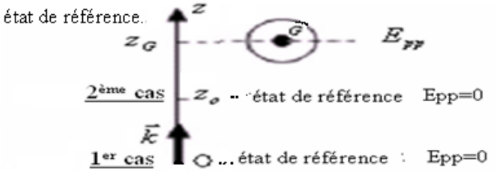
\includegraphics[width=0.5\textwidth]{./img/img00.png}
%\end{wrapfigure}

%\begin{center}
   %\begin{tabular}{ |c|c|c|c|c|c|c| }
      %\hline
      %km & hm & dam & \bf{m} & dm & cm & mm \\
      %\hline
        %&   &    &  &   &   & \\
%\hline
%\end{tabular}
%On place un seul nombre dans chaque case.
%\end{center}
%\begin{center}
   %\begin{tabular}{ |c|c|c|c|c|c|c| }
      %\hline
      %$km^2$ & $hm^2$ & $dam^2$ & \bf{$m^2$} & $dm^2$ & $cm^2$ & $mm^2$ \\
      %\hline
        %&   &    &  &   &   & \\
%\hline
%\end{tabular}
%\end{center}


\end{document}

